\documentclass{ferseminar}
\student{Toma Šimunić}
\voditelj{prof.~dr.~sc. Ivana Podnar Žarko}
\mjestodatum{Zagreb}{April}{2018}
\naslov{Implementing cryptocurrency NANO\\ as payment option in e-commerce}
\usepackage{graphicx}
\graphicspath{ {images/} }
\begin{document}
\stvoripredstranice
\section{Introduction}
Commerce is an activity of buying and selling. Currencies are arbitrary representations of value which are used in commerce since prehistoric ages. The evolution of currencies can be described in a linear progression:

\begin{enumerate}
	\item Early currencies
	\item Coinage
	\item Paper money
	\item Digital currencies
\end{enumerate}

Blockchain technology and the Proof-of-Work concept made digital currencies possible. With the emergence of digital currencies, from now on referred to as cryptocurrencies, some e-commerces started implementing different cryptocurrencies as payments options. Due to their price volatility, cryptocurrencies present a risk to the merchant, but on the other hand provide a few reasons for adopting the new payment option.

One of the motivations for implementing cryptocurrency payment options is to attract new customers by providing a new solution. Cryptocurrency enthusiasts often look for shops that accept their currency and shops gain loyal customers this way. Another motivation is that the fees for processing transactions are much lower using some cryptocurrencies than conventional card payment options.

The first, and most popular, cryptocurrency, Bitcoin, was released in 2009. as an open-source software by Satoshi Nakamoto. Since then, Bitcoin has gained a lot in value and has seen some adoption by e-commerces, as well as regular commerces. The increase in Bitcoin's price had a negative impact on it's adoption as a currency because it resulted in transaction fees rising above those of using a credit card. This phenomenon has increased the need for an alternative solution.

Cryptocurrency Nano was first introduced in 2014. It stands out from other cryptocurrencies for having fee-less and instant transactions, which is made possible by using the block-lattice structure. This makes it a viable contestant for use in e-commerce.

In this paper, I will analyze and compare conventional payment processes, payment processes using a third-party and Peer-to-Peer payment processes using PayPal, Bitcoin and Nano as examples.


\section{E-commerce payment systems}

Consumer spending via the internet has seen a significant increase in the last decade. By expanding their business online, merchants increase their market reach. Online payment systems can be broadly defined as the means and processes involved in conducting transactions online \cite{Lowry}. Advantages of paying online include:
\begin{itemize}
	\item improved cash flow efficiency - websites are a cost effective way of collecting funds
	\item guaranteed transactions - payment providers offer customers assurance by maintaining high-quality equipment and implementing protection policies to gain trust
	\item reduced cost - online payments reduce cost on both the business and client side of a transaction
	\item increased protection of sensitive information - decreases chance of internal employee theft
	\item increased protection of payment providers - online payment providers assume the risk of fraud
\end{itemize}

The possibility of fraud makes security a priority in online payment systems. Most important security aspects are: identification, confidentiality, authentication, data integrity, non-repudiation and	customer solvency.

Merchant's discount is a term used in e-commerce to represent the fee that is being payed to the payment processors. The merchant deducts the fee from the price of the product. With most payment processors it averages in around 3\%. That is the cost of having secure credit card payments, both online and offline. 

There are three major types of online payment systems:
\begin{enumerate}
	\item conventional payment processing
	\item third-party payment providers
	\item Peer-to-Peer payment
\end{enumerate}

\subsection{Conventional payment processing}
To accept an online payment, a merchant has to obtain an account from a bank and program the interaction with a credit card payment processor. The components interacting are customer, merchant, merchant's bank and credit card issuer.

A \textbf{merchant's account} is a credit card account capable of receiving funds from his online customers. It easier, more economical and convenient to establish a merchant account with someone that provides payment gateway

\textbf{Shopping cart software} is used to maintain a link between a customer and his set of selected items by allowing him to store items in the cart. It serves as a link between the merchant and the credit card processing network.

A \textbf{payment gateway}, also referred to as payment processor, connects the shopping cart with the merchant's bank and the customer's bank. It is a key component of online transactions. The payment gateway first verifies the credit card information. If everything is confirmed by the credit card company, an approval is sent to the payment gateway which communicates the confirmation with the shopping cart. Then, a payment settlement is initiated to transfer funds from the customer's to the merchant's account. The whole process is represented in Figure 1.
\begin{figure}[p]
	\caption{Conventional payment processing diagram}
	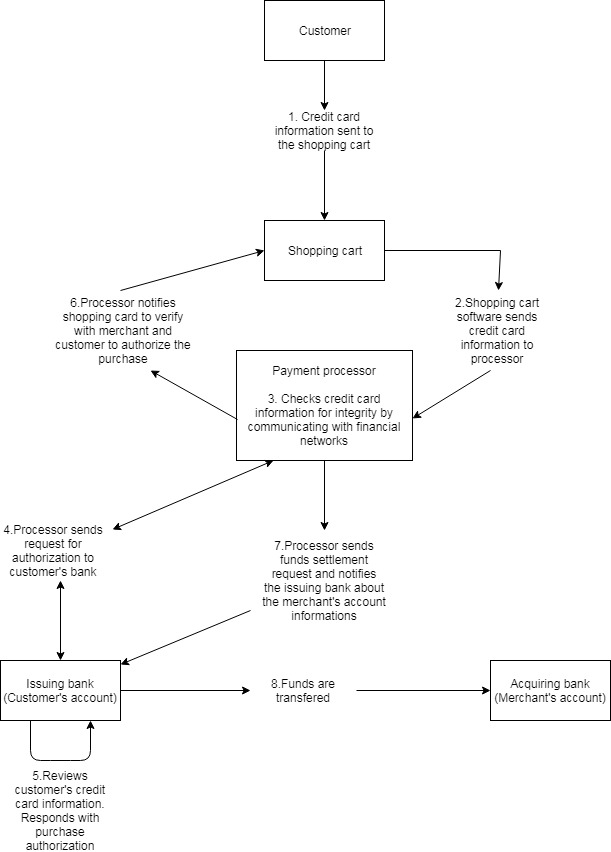
\includegraphics[scale=0.7]{diagram1}
	\centering
\end{figure}


\subsection{Third-party payment providers}

The third-party online payment process is similar to the conventional payment system. In this system, the third-party processes all the transaction funds so there is no need for a merchant credit card account. The system is shown in Figure 2. 

The \textbf{shopping cart} is still responsible for maintaining a connection between the customer and the selected items. When finished shopping, the customer is forwaded to a webpage maintained by the third-party payment provider to collect credit card information.

The \textbf{payment} gateway authorizes the transaction and holds the funds in trust for the merchant. Transfer to the merchant's local bank account occurs on a regular basis, predetermined in the subscription contract.

\begin{figure}[t]
	\caption{Third-party payment processing diagram}
	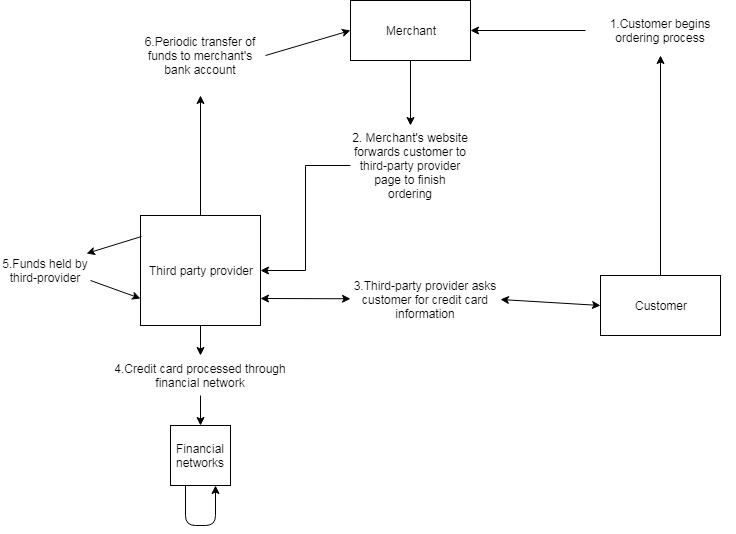
\includegraphics[scale=0.6]{diagram2}
	\centering
\end{figure}

\subsection{Peer-to-Peer payment}

Peer-to-Peer payment is a form of online payment that provides an inexpensive way to accept online payment services. PayPal is recognized as the most prominent among the P2P payment services. PayPal was established in 1998 and is owned by eBay since 2002. For a P2P service to work, both the merchant and the customer need to have an account with the same P2P provider because the payment process is handled internally through the P2P provider. Figure 3. shows a typical P2P transaction.

There are a few differences between PayPal's P2P solution and cryptocurrencies. First, PayPal uses a fixed fee equaling around 3\% per transaction while cryptocurrencies have fixed fees or no fees in the case of Nano. The second difference is that PayPal is directly connected to their users bank accounts to charge users while trading with cryptocurrencies is direct from the customer to the merchant. Both systems require high-level security management. 
\begin{figure}
	\caption{Peer-to-Peer payment processing diagram}
	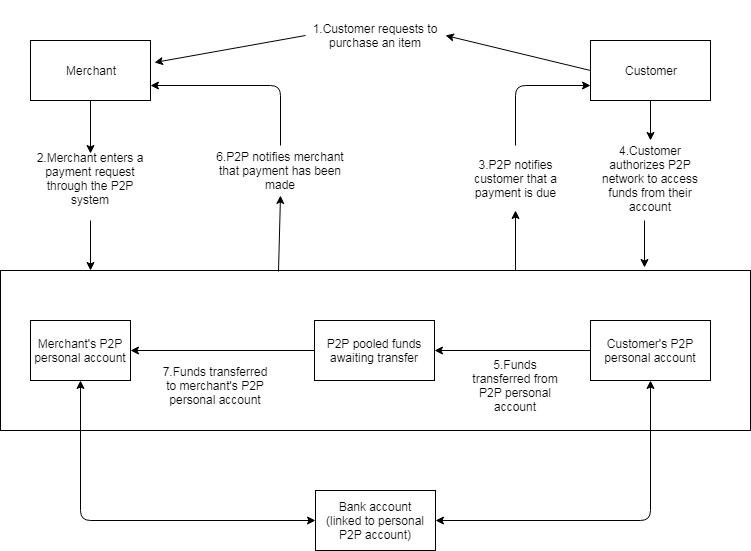
\includegraphics[scale=0.6]{diagram3}
	\centering
\end{figure}


\section{Bitcoin in e-commerce}

\subsection{About Bitcoin}
Bitcoin is a cryptocurrency developed by Satoshi Nakamoto and published as an open-source software in 2009. It uses a blockchain data structure for storing transaction information and a Proof-of-Work consensus protocol to secure the validity of the transactions, making them tamper-proof. It allows online payments to be sent directly, peer-to-peer, without going through a financial institution and the consensus mechanism is based on cryptographic proof instead of trust.

\subsection{Bitcoin performances}
Bitcoin's network produces one block every 10 minutes, each block containing 1 MB. That makes the Bitcoin network average in around 7 transactions-per-second. Transactions that have offered the highest processing fee for transactions will be processed first.


\subsection{Bitcoin in e-commerce}
When Bitcoin was first introduced, it was proposed as a solution to on-line payments without requiring an intermediary between the customer and the merchant, cutting the costs of transactions in the process. This was favourable to both customers and merchants, which made it popular in e-commerce. However, for the payments to be processed a checkout application must be in place to monitor the payment for the specific product or list of products. This requires either programming skills or a third-party payment processor. The payment process is similar to the one described in Figure 3. without using bank accounts. Instead, both merchant and customer are the primary owners of their accounts and therefore settle transactions without bank accounts.

Most recently, Bitcoin has seen a negative adoption trend, it was discarded by the world's largest gaming platform \textit{Steam}. It is speculated that the reasons were high volatility and high transaction fees. During December, 2017. Bitcoin's fees went up to a price of around 52 USD per transaction, making it a luxury to pay in Bitcoin. Transaction fees have decreased from then on, today being 1.3 USD. This still represents a problem for average Bitcoin users.


\subsection{Third-party payment processors}
Third-party payment processors are specialized in providing tools to integrate Bitcoin payment option into your website. 

\subsubsection{Coinbase}
Coinbase is a Bitcoin payment processor that offers 0\% fees for the first million USD in transactions and 1\% fee after. It is only available for US bank accounts and offers a simple website integration.
\subsubsection{BitPay}
BitPay is an international payment processor for businesses and charities. BitPay works with Amazon, allowing merchants to sell and ship items through Amazon using cryptocurrencies. It requires a 1\% fee or a monthly fee of 3000 USD.
\subsubsection{BIPS}
Short for the Bitcoin Internet Payment System, it allows merchants to buy and sell Bitcoin for 0\% fees. It also offers an easy-to-use mobile checkout app and a point-of-sale for commerces without internet shops.
\subsection{Pros and Cons for using Bitcoin in e-commerce}
\subsubsection{Pros}
There are \textbf{no chargebacks} with Bitcoin payment. Once a transaction is confirmed the funds are transfered and the order shipped.

\textbf{You determine the transaction fees.} Transaction fees are flexible and depend on the busyness of the transaction pool. If your transaction doesn't have the need to be processed quickly, you can pay a much lower fee.

\textbf{Anonymity.}Bitcoin addresses aren't tied to your identity. However, by thoroughly investigating transactions tied to a particular public key, one can conclude who is the owner.

\subsubsection{Cons}
\textbf{Price volatility.} Bitcoin, like most cryptocurrencies, is a speculative asset. It can double or halve it's worth in a single day, making either customer or merchant unhappy with the transaction.

\textbf{Security.} Bitcoin is a novelty in the technological worth so there are still ways that can ease the use of it as a currency to the average user. Banks hold your money for a price but offer security. By safekeeping your own money you take the risk of doing so. 

\textbf{Speed.} In the Bitcoin network, one block is mined every 10 minutes, averaging in 7 transactions-per-second. This makes customers wait for 10 minutes, if the prioritize this transaction with high fees, to have their orders confirmed.

\textbf{Transaction fees.} Transaction fees are volatile and are entirely dependent on mining pools that can raise the fee at any moment. In the cryptocurrency-sphere there is a rule of thumb for establishing if the fees of a currency are too high. If you wouldn't pay for coffee with the currency, the fees are too high.

\textbf{Power inefficiency.} The Bitcoin network consumes an estimated 27.28 TWh per year using an average 260 KWh for a transaction \cite{Nano}.

\section{Nano cryptocurrency}

NANO is a low-latency cryptocurrency introduced in December, 2014. as Raiblocks by Colin LeMahieu. It is one of the first Directed Acyclic Graph (DAG) cryptocurrencies built on an innovative block-lattice data structure which offers unlimited scalability and no transaction fees. Nano is a simple protocol by design and only has the purpose of being a high-performance cryptocurrency. Nano and Bitcoin differ in many aspects which will be presented in this chapter.

\subsection{Nano components}
The overall Nano architecture consists of four individual components:
\begin{itemize}
	\item Account
	\item Block/Transaction
	\item Ledger
	\item Node
\end{itemize}

\subsubsection{Account}
An account is the public-key of a digital signature key-pair. The account's public-key also serves as the account's address and is publicly available while the private-key is kept secret. By signing a packet it is ensured that the contents were approved by the private-key holder. 

\subsubsection{Block/Transaction}
In the Nano network each block contains only one transaction. A transaction is an action while the block is the digital encoding of the transaction.

\subsubsection{Ledger}
The ledger is the global set of accounts where each account has its own transaction chain. It is stored on Nano network nodes.

\subsubsection{Node}
A node is a piece of software running on a computer that conforms to the Nano protocol and participates in the Nano network. The node may either store the entire ledger or a pruned history containing only the last few blocks of each account's blockchain.  

\subsection{System overview}

Nano uses a block-lattice structure which makes it the first cryptocurrency to do so. In the block-lattice structure every account has its own blockchain which is equivalent to the account's transaction history. The account-owned blockchain can only be updated by the private key owner. The nodes in the network are designated to keep the account's balance in check. Some nodes are uninterested in keeping the whole transaction history of an account so they store only the last transaction.

Each transaction in the Nano protocol is small enough to fit into a UDP packet. This feature gives the Nano network low-latency. Currently, there are four transaction types: 
\begin{itemize}
	\item open
	\item send
	\item receive
	\item change
\end{itemize}
They will soon be replaced by a Universal transaction which will keep each account's blockchain smaller and will allow easier ledger prunning. Prunning is a process of minimizing the ledger size by deleting redundant information. 

\subsection{Nano performance}
Nano offers near-instant transactions and does that without requesting fees. The Nano test-network scaled to 10000 transactions-per-second while the main-network has been tested on 300 transactions-per-second.


\section{NANO in e-commerce}
Analysis of e-commerce trends have shown that there are three areas that can potentially increase the use of online payments:
\begin{itemize}
	\item micropayments
	\item mobile payments
	\item distributed payment systems
\end{itemize}

\textbf{Micropayments} are small electronic payments. The difficulty in implementing micropayments is in charging transaction fees which can possibly be greater than the payment itself.

\textbf{Mobile payments} are payments made from a mobile phone. Prior to the emergence of smartphones, researchers were investigating the potential use of mobile devices in short range wireless networks for commerce. With current technology, mobile devices have the ability to reach and interact any website available on the World Wide Web. In addition, many cryptocurrency wallets offer smartphone applications which provides a better solution than the short range wireless networks that were investigated in 2006.  

Leaving a centralized client-server payment system and making a \textbf{Peer-to-Peer distributed electronic system} (P2P)can grant many benefits. The payment processors require fees which can be drastically decreased or removed in a P2P system.

\textbf{Nano} is capable of fulfilling all of those requests. \textbf{Micropayments} are made possible by the non-existence of transaction fees, the low latency of the network and high scalability. \textbf{Mobile payments} will be possible with the final release of the Android and iOS wallets \textit{(do završne verzije seminara ću vrlo vjerojatno promijenit ovaj dio, trenutno su walleti u završnoj beta fazi)}.Nano is a \textbf{P2P distributed electronic system} which makes every member of the Nano network their own bank. The transactions don't need to be mediated by third-parties which in synergy with non-existent fees make it a perfect match for e-commerce use.
\subsection{Payment gateways}






\section{Conclusion}
The three payment methods analyzed in this paper all have their pros and cons. While the cryptocurrency options leave you in control of your money, they are not universally accepted in e-commerce. The challenge for cryptocurrencies is mass adoption. For mass adoption to be possible, they have to bring greater value to the table than their competitors. Some e-commerces have made the decision to open their market for cryptocurrencies to attract new customers. This was mostly done by small e-commerces because they have a higher incentive to take risks. 


\begin{center}
	\begin{tabular}{ |c||c|c|c| }
		\hline
		& Conventional e-commerce & Bitcoin & Nano\\ 
		\hline\hline
		Fees & 3\% & Volatile & None\\  
		\hline
		Transaction speed & Seemingly instantaneous & 10 minute & Near-instant\\
		\hline
		Network scalability (tx/s) & 24000 & 7 & 300\\
		\hline
	\end{tabular}
\end{center}
\dodajliteraturu{bazaLiterature}
\section{Abstract}
\end{document}
